\renewcommand{\bs}[1]{\boldsymbol{#1}}
\newcommand{\mb}[1]{\mathbf{#1}} 
\newcommand{\mc}[1]{\mathcal{#1}} 
\newcommand{\mbb}[1]{\mathbb{#1}} 
\newcommand{\txt}[1]{\texttt{#1}} 
\newcommand{\pdiff}[3]{ \if 1#1 
	\frac{\partial #2}{\partial #3} \else \frac{\partial^{#1} #2}{\partial 
		#3^{#1}}\fi}
\newcommand{\ppdiff}[3]{\frac{\partial^2 #1}{\partial #2 \partial #3}}
\newcommand{\sdiff}[3]{ \if 1#1 \frac{d #2}{d #3} \else \frac{d^{#1} #2}{d 
		#3^{#1}}\fi}
\newcommand{\e}{\mbox{e}}
\newcommand{\rvec}[1]{\overrightarrow{#1}}
\newcommand{\uvec}[3]{#1\,\mb{i}~ #2\,\mb{j}~ #3\,\mb{k}}

\subsection{MATLAB}
\begin{frame}{\txt{MATLAB}}
\begin{itemize}
	\item \txt{MATLAB} is a high-level language and interactive environment for numerical computation,
	visualization and programming.
	\begin{itemize}
		\item Analyze data
		\item Develop algorithms
		\item Create models and applications
	\end{itemize}
	\item We will reinforce some calculus concepts and its applications using \txt{MATLAB}, such as
	\begin{itemize}
		\item Numerical differentiation
		\item Numerical Integration
		\item Root-finding methods
	\end{itemize}
\end{itemize}
\end{frame}

\begin{frame}{Software}
\txt{MATLAB} is installed in the campus computer labs. 
However, if you wish to work from home or on your laptop, you can either
\begin{enumerate}
	\item use \txt{MATLAB} Online on your web browser; or
	\item install \txt{MATLAB} on your personal computer. 
\end{enumerate}

\begin{alertblock}{MATLAB Campus-wide suite}
To install or use \txt{MATLAB} on your web browser, you need to create a Mathworks
account using your UBD e-mail. You can access the UBD campus-wide suite using your mathworks account.\\
Please refer to the \txt{MATLAB} individual CWL installation guide document.
\end{alertblock}
\end{frame}

\begin{frame}{MATLAB Online}
\begin{center}
	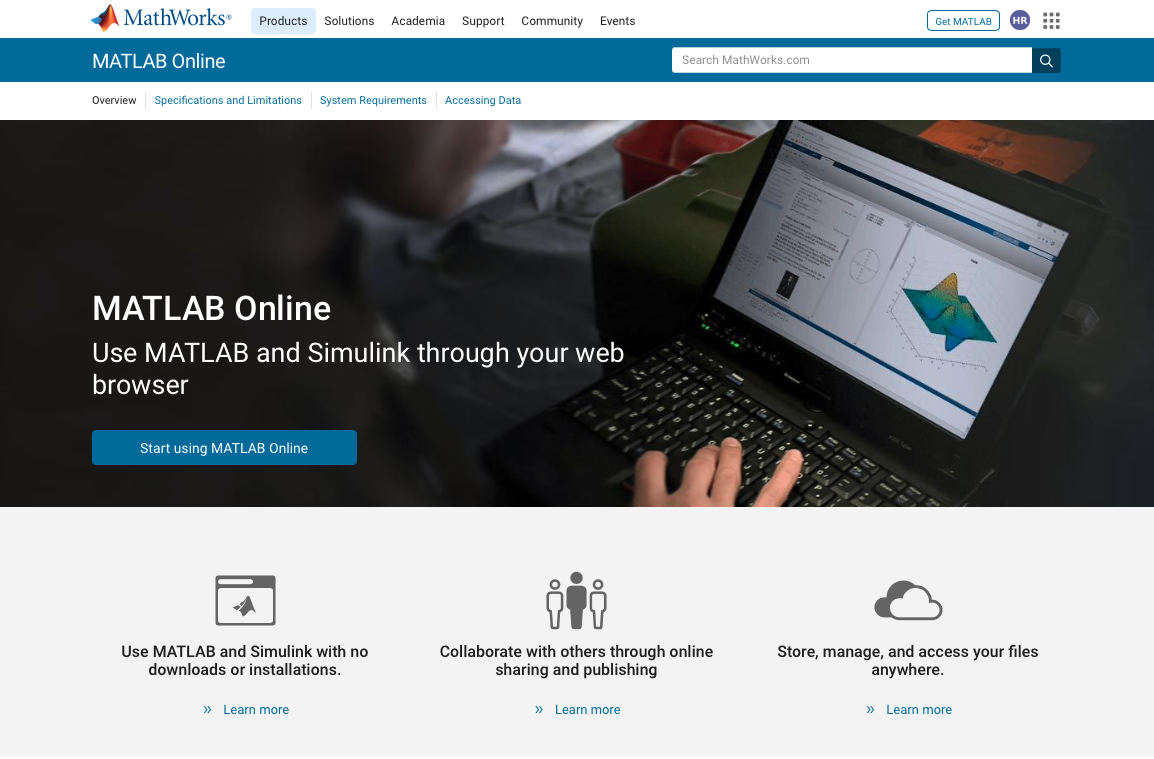
\includegraphics[width=0.6\textwidth]{matlab_online}
\end{center}
\url{https://matlab.mathworks.com}
\end{frame}



\begin{frame}{MATLAB Graphical Interface}
\begin{columns}
\begin{column}[T]{0.35\textwidth}
\begin{itemize}
	\item Command window
	\item Workspace
	\item Current folder
	\item Command history
	\item Editor
	\end{itemize}
\end{column}
\begin{column}[T]{0.75\textwidth}
	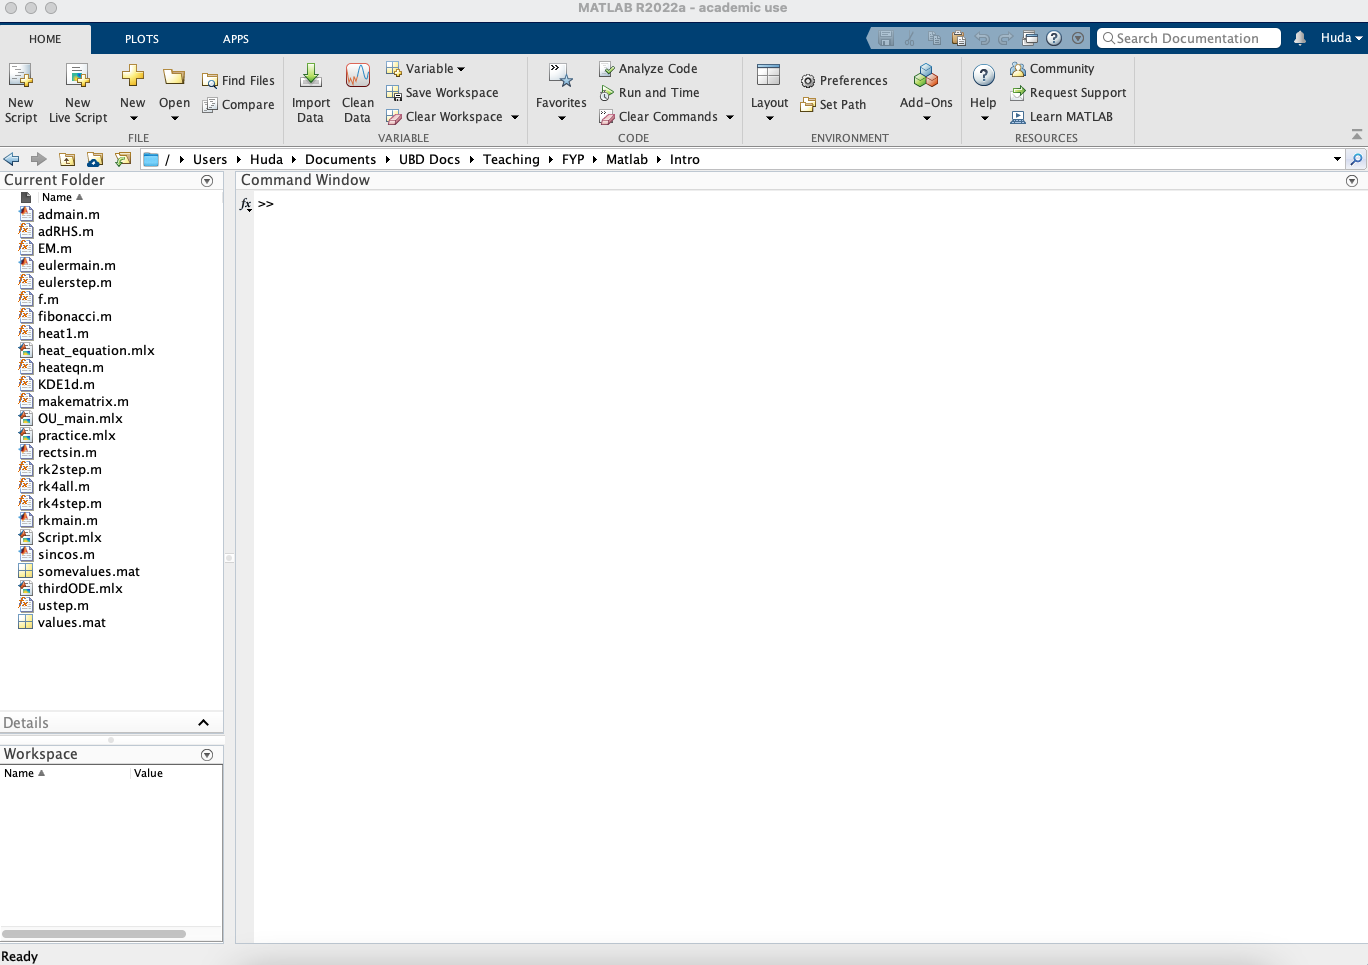
\includegraphics[width=0.85\textwidth]{initial_matlab}
\end{column}
\end{columns}

\end{frame}

